\section{Preliminary Production Results}\label{sec:preliminary}

\subsection{Implementation and protocol}

The method is implemented in the production balanced Newton path of the
HySim-XJTU-HRPES C++20 codebase. All preliminary timings use an AppleClang 21
arm64 macOS Release build with KLU. The Schur benchmark parses each case once,
performs two warmups, and then executes five alternating full/Schur solves. The
reported times are medians. The benchmark forces Schur on case300 for research
ablation even though the production admission rule excludes it.

The current KLU adapter does not report factor nonzeros or factor work. Those
fields are explicitly marked unavailable; the results below report input
structural nonzeros, dimensions, iterations, and measured time without
fabricating fill statistics.

\subsection{Functional and numerical verification}

The registered VSC-limit suite passes 45 cases and 540 assertions. Its scope is
summarized in Table~\ref{tab:verification}. Analytic generalized Jacobians are
checked by finite differences away from switching ties, and the biactive
Fischer--Burmeister origin is tested without a hidden perturbation.

\begin{table*}[t]
\caption{Current verification coverage and acceptance boundaries}
\label{tab:verification}
\centering\footnotesize
\setlength{\tabcolsep}{4pt}
\begin{tabular}{p{0.19\textwidth}p{0.47\textwidth}p{0.25\textwidth}}
\toprule
Category & Covered cases & Acceptance evidence\\
\midrule
Local equations
& Magnitude, P-first, and Q-first power ports; all three GFM priorities;
Vdc-droop saturation; zero-radius and biactive intersections
& Local/oracle and exact complementarity residuals at most $10^{-9}$;
biactive residual at most $2\times10^{-15}$\\
Analytic derivatives
& Local power-port and GFM terminal/internal-voltage derivatives; smooth FB and
smoothed median derivatives
& Centered finite-difference discrepancy at most $5\times10^{-7}$\\
Network integration
& Two simultaneous power-port limits, two simultaneous GFM limits, weak-grid
roots, and deliberately infeasible weak-grid points
& One fixed Jacobian-pattern build; infeasible points are not reported as
converged\\
Cross-process consistency
& Three-step quasi-steady replay, balanced OPF dispatch replay, stable-ID JSON
round trip, GFM-island extraction, and transient initialization
& OPF-to-PF exact certificate at most $10^{-9}$; PF-to-transient Norton seed
errors at most $10^{-8}$\\
External circuit validation
& Nonbinding GFM Thevenin point and binding frozen-internal-voltage circuit in
OpenDSS
& Nonbinding $|\Delta V|\le10^{-4}$ p.u.; binding native terminal KCL residual
at most $10^{-6}$ p.u.\\
\bottomrule
\end{tabular}
\end{table*}

The OpenDSS evidence has two levels. At the nonbinding point, OpenDSS solves an
equation-equivalent two-source Thevenin circuit independently. At the binding
point, OpenDSS has no native equivalent of the proposed priority-NCP control;
the internal voltage obtained by HySim is frozen and the external circuit is
re-solved. The latter validates the electrical circuit and terminal KCL, but it
is not an independent mode-selection oracle.

The focused transient initialization filter passes four cases and 51
assertions. It verifies stable-ID transfer of internal voltage, terminal
current, and terminal power before dynamic network trimming, including a
slackless GFM island. The maximum accepted seed error for each quantity is
$10^{-8}$ p.u. A later dynamic trim may move the equilibrium when the dynamic
device set does not reproduce the steady-state slack dispatch, so this result
is an initialization consistency certificate rather than a transient-stability
claim.

\subsection{Schur algebraic oracle}

A small sparse algebraic oracle compares the Schur step with a direct complete
LU solution. The relative step error is at most $10^{-10}$ and the reconstructed
complete-system backward error is at most $10^{-12}$. A singular selected local
block is rejected, and an integration test forces the production solver to
fall back to complete sparse LU while retaining convergence.

For the network benchmarks, Schur and full-LU solutions satisfy
\begin{equation}
 \|\Delta V\|_{\infty},\quad
 \|\Delta\theta\|_{\infty},\quad
 \|\Delta V_{\dc}\|_{\infty}
 \le10^{-8}.
\end{equation}
This establishes numerical equivalence of the converged roots within the
declared tolerance; it does not assert uniqueness of the nonlinear root.

\subsection{Large hybrid benchmark results}

The case300 benchmark contains 300 ac buses, six dc buses, and six explicit
VSC blocks. ACTIVSg2000 contains 2000 ac buses, eight dc buses, and eight VSC
blocks. Each case has four simultaneous binding power-port limits. These are
real hybrid networks rather than pure-ac cases with timing labels added after
the fact.

Figure~\ref{fig:benchmark-results} presents the measured structure, timing,
and certificate outcomes before the exact values are tabulated. It makes the
production crossover visible: the same reduction is detrimental on case300
but beneficial on ACTIVSg2000. It also shows that the large-case speedup is
obtained while rejecting numerically inadmissible Schur steps rather than
silently accepting every reduced solve.

\begin{figure*}[t]
\centering
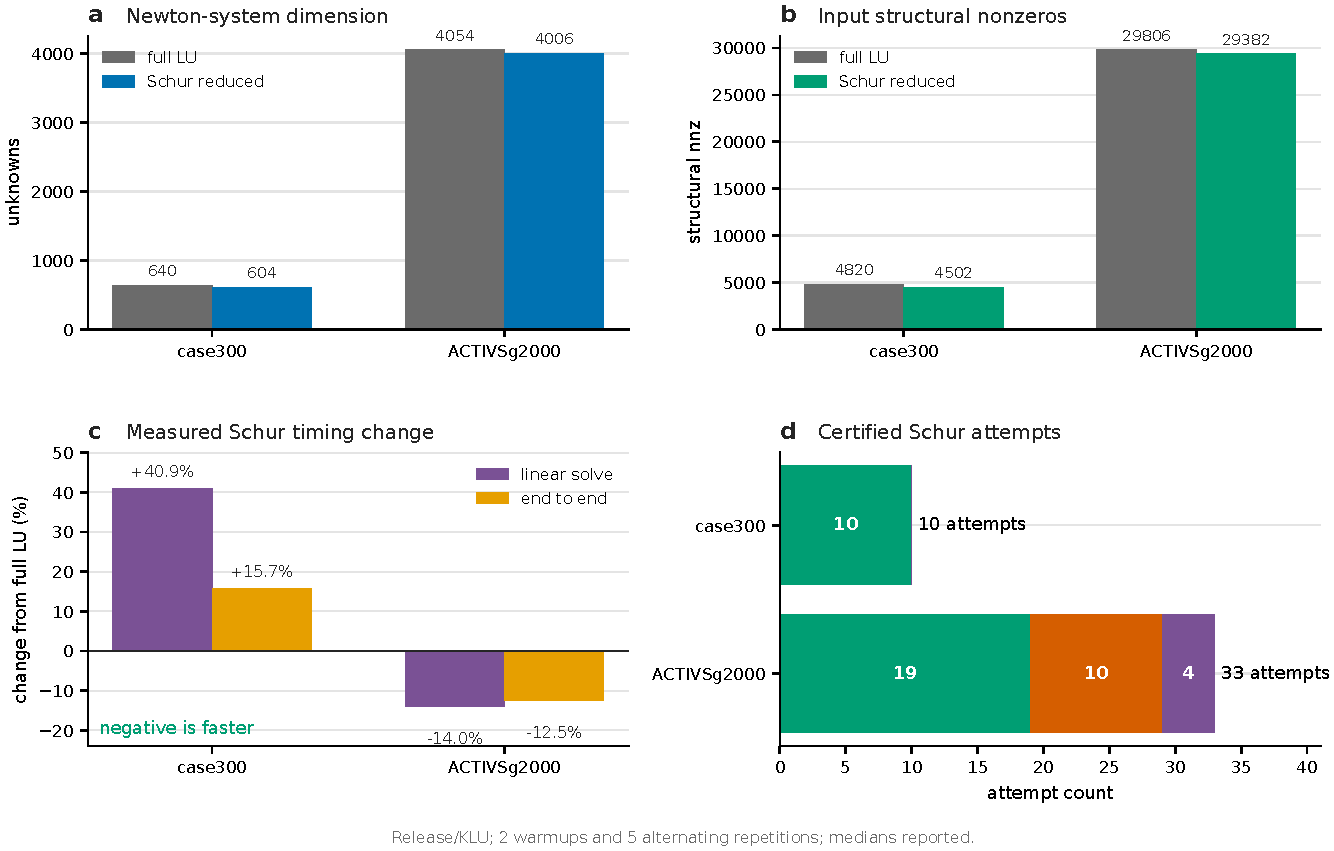
\includegraphics[width=0.94\textwidth]{figures/benchmark_results.pdf}
\caption{Production CPU/KLU Schur benchmark using the fixed two-warmup,
five-repeat alternating protocol. (a) Full and reduced Newton dimensions.
(b) Input structural nonzeros; factor-fill statistics are unavailable from the
current adapter and are not inferred. (c) Median timing change relative to
complete sparse LU, where negative values indicate acceleration. (d) Accepted
and rejected Schur attempts: green denotes accepted steps, orange denotes
local-regularity rejection, and purple denotes reconstructed full-step
backward-error rejection. case300 is a forced research ablation; the production
admission rule excludes it.}
\label{fig:benchmark-results}
\end{figure*}

Figure~\ref{fig:benchmark-results}(a)--(b) confirms the structural predictions: six
states are removed per VSC, and the observed structural reductions exceed the
$48m$ lower bound. It also demonstrates why structure preservation must be
measured rather than assumed. On case300, local factorization and certificate
overhead dominate the small network factorization, so forced Schur is slower.
On ACTIVSg2000, the reduced factorization is large enough to offset the local
work, lowering both linear and end-to-end median time.

The full/Schur median linear and wall times are respectively
$0.491/0.692$~ms and $2.675/3.094$~ms for case300, and
$31.561/27.135$~ms and $47.391/41.486$~ms for ACTIVSg2000. Thus the
visual percentage changes in Fig.~\ref{fig:benchmark-results}(c) retain their
underlying absolute measurements without requiring a duplicate wide table.

For case300, all ten Schur attempts are accepted. The minimum accepted local
$rcond$ is $5.48\times10^{-2}$ and the maximum accepted full backward error is
$3.63\times10^{-17}$. For ACTIVSg2000, 19 of 33 Schur attempts are accepted;
ten are rejected by the local-regularity guard and four by the reconstructed
full backward-error guard. The minimum accepted local $rcond$ is
$2.19\times10^{-8}$, and the maximum accepted full backward error is
$5.96\times10^{-17}$. Rejected attempts use the complete sparse-LU path rather
than terminating the nonlinear solve.

\subsection{Interpretation and present limitations}

The preliminary evidence supports three current claims: the explicit NCP
model remains structurally fixed across activation; the local Schur solve is
algebraically equivalent when its certificate is accepted; and a measurable
CPU benefit appears on the tested 2000-bus hybrid case. The evidence does not
yet support a universal crossover dimension, GPU acceleration, sparse-factor
fill reduction, or large-scale simultaneous binding GFM behavior. The default
dimension of 1000 is therefore exposed as configurable policy and is not
treated as a theorem.

The large GFM datasets currently add one nonbinding Norton GFM block to a
certified MTDC operating point through continuation. They verify data/model
integration and fixed structure, but not flat-start robustness or simultaneous
large-scale GFM limiting. Likewise, weak-grid cases exercise difficult local
roots but do not replace a systematic CPF continuation toward a voltage-
stability nose. These experiments define the remaining work needed before the
results section is submission complete.
